% Industrialization -> bone DAG (Supplementary Figure 3), TikZ standalone.
% Matches the visual grammar of the other DAG figures here: Inter sans, stage-fill palette, rounded nodes, red confounder
% edges, green causal edge, grey mediator edges, red MSAS nodes.
%
% Structure: industrialization (exposure) -> bone (outcome). Age + sex are the ONLY
% confounders (MSAS, red); daily physical activity, fat/lean mass, pregnancy/lactation,
% and smoking/alcohol are MEDIATORS downstream of industrialization (grey, not adjusted)
% -- the reason the minimal sufficient adjustment set is just {age, sex}.
%
% Build (xelatex; run twice):
%   xelatex urb-bone.tex
% Output: urb-bone.pdf -> outputs/figures/final/supp-fig-3-urb-dag.pdf

\documentclass[border=10pt]{standalone}
\usepackage{fontspec}
% BoldFont declared so the legend's \textbf{Nodes:}/\textbf{Edges:} resolve --- plain
% "Inter" ships no bold shape here, so the bold face is named explicitly.
\setsansfont{Inter}[BoldFont={Inter 18pt SemiBold}]
\renewcommand{\familydefault}{\sfdefault}
\usepackage{tikz}
\usetikzlibrary{arrows.meta, positioning, fit, backgrounds, calc}

\definecolor{stageSetup}{HTML}{CFD8EA}   % outcome
\definecolor{stageLang}{HTML}{CFDFCD}    % exposure
\definecolor{stageAuth}{HTML}{E3C2BC}    % adjustment set
\definecolor{dark}{HTML}{1E293B}
\definecolor{slate}{HTML}{64748B}
\definecolor{linegreen}{HTML}{3F7E4E}    % causal edge
\definecolor{linered}{HTML}{A85D52}      % confounder edges / MSAS border

\tikzset{
  font=\sffamily\footnotesize,
  exposure/.style={rectangle, rounded corners=4pt, draw=slate!75, line width=0.7pt,
                   fill=stageLang, text=dark, align=center, minimum width=2.1cm, minimum height=0.95cm},
  outcome/.style={rectangle, rounded corners=4pt, draw=slate!75, line width=0.7pt,
                  fill=stageSetup, text=dark, align=center, minimum width=1.7cm, minimum height=0.95cm},
  msas/.style={rectangle, rounded corners=4pt, draw=linered, line width=0.9pt,
               fill=stageAuth, text=dark, align=center, minimum width=1.4cm, minimum height=0.9cm},
  obs/.style={rectangle, rounded corners=4pt, draw=slate!75, line width=0.7pt,
              fill=white, text=dark, align=center, minimum width=1.8cm, minimum height=0.9cm},
  causal/.style={-{Latex[length=2.6mm]}, draw=linegreen, line width=1.4pt},
  conf/.style={-{Latex[length=2.6mm]}, draw=linered, line width=1.0pt},
  other/.style={-{Latex[length=2.6mm]}, draw=slate, line width=0.6pt, opacity=0.85},
  anno/.style={font=\sffamily\itshape\small, text=slate},
  legend/.style={font=\sffamily\scriptsize, text=dark, align=center},
}

% ---- legend helpers ----
% The swatch macros take a style/colour name, so they resolve against THIS file's own
% \tikzset above -- the legend therefore cannot drift from what is drawn. The legend
% sits below the caption, so the standalone bounding box grows downward only.
% Vertical centring is set PER SWATCH TYPE, and each value was swept INSIDE this
% figure and measured at 1200 dpi against its own adjacent label. A single shared
% knob does not work here: the three macros build different objects (a tikz node, a
% plain rule, a tikz path) and they do not land alike for a given offset in this
% file's context. If they need retuning, sweep them in the figure itself: a reduced
% test case lacks the global font= in \tikzset that the nested \tikz swatches inherit,
% and will centre them correctly there while leaving them ~3 pt low here.
\newcommand{\swnode}{-1.5ex}                       % \lnode  (tikz node)
\newcommand{\swdash}{-0.65ex}                      % \ledgedash (tikz path)
\newcommand{\swrule}{\dimexpr0.5ex-0.55pt\relax}   % \ledge (rule lift, from its bottom)
\newcommand{\lnode}[1]{\tikz[baseline=\swnode]\node[#1, minimum width=0.38cm, minimum height=0.24cm, inner sep=1.5pt]{};}
\newcommand{\ledge}[1]{{\color{#1}\rule[\swrule]{0.5cm}{1.1pt}}}
% Entry wrappers: \mbox keeps a swatch glued to its label so the line can only break
% BETWEEN entries, never inside one.
\newcommand{\lentry}[2]{\mbox{\lnode{#1}\ #2}}
\newcommand{\eentry}[2]{\mbox{\ledge{#1}\ #2}}

\begin{document}
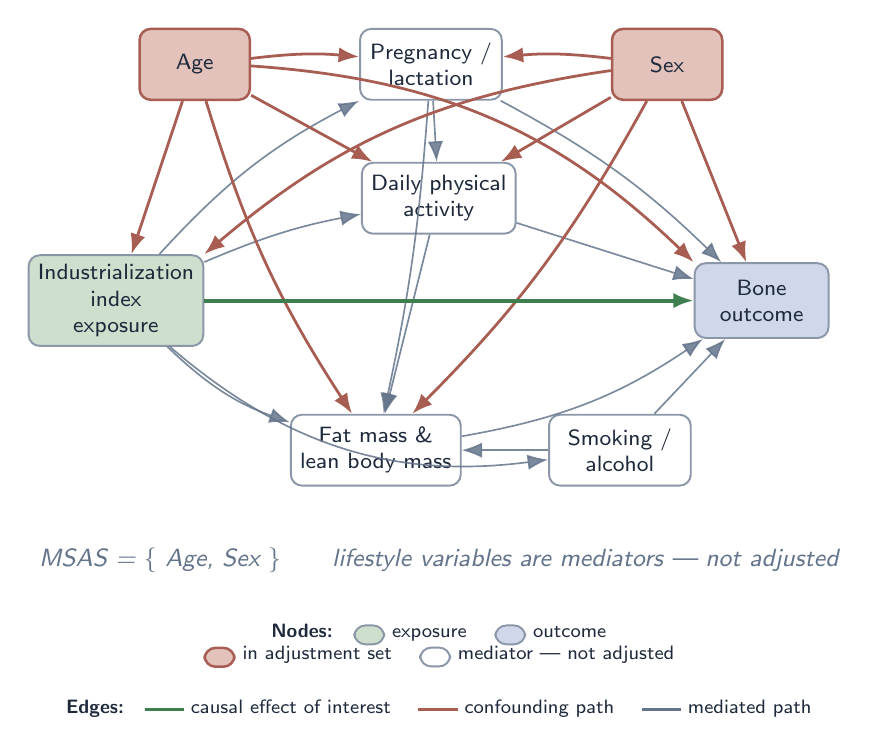
\begin{tikzpicture}
  % --- nodes (exposure left, outcome right; green axis kept clear) ---
  \node[exposure] (urb)     at (0.6, 2.6)  {Industrialization\\ index\\ exposure};
  \node[outcome]  (osteo)   at (8.8, 2.6)  {Bone\\ outcome};
  \node[msas]     (age)     at (1.6, 5.6)  {Age};
  \node[msas]     (sex)     at (7.6, 5.6)  {Sex};
  \node[obs]      (pl)      at (4.6, 5.6)  {Pregnancy /\\ lactation};
  \node[obs]      (dpa)     at (4.7, 3.9)  {Daily physical\\ activity};
  \node[obs]      (fatlean) at (3.9, 0.7)  {Fat mass \&\\ lean body mass};
  \node[obs]      (smk)     at (7.0, 0.7)  {Smoking /\\ alcohol};

  % --- grey mediator-chain edges (industrialization -> lifestyle vars -> bone) ---
  \draw[other] (urb) to[bend left=6]  (dpa);
  \draw[other] (urb) to[bend right=12] (fatlean);
  \draw[other] (urb) to[bend left=10] (pl);
  \draw[other] (urb) to[bend right=24] (smk);
  \draw[other] (dpa) -- (osteo);
  \draw[other] (dpa) -- (fatlean);
  \draw[other] (fatlean) to[bend right=12] (osteo);
  \draw[other] (pl) to[bend left=8] (osteo);
  \draw[other] (pl) -- (dpa);
  \draw[other] (pl) to[bend left=4] (fatlean);
  \draw[other] (smk) -- (osteo);
  \draw[other] (smk) -- (fatlean);

  % --- red confounder edges: {age, sex} -> {exposure, outcome, mediators} ---
  \draw[conf] (age) -- (urb);
  \draw[conf] (age) to[bend left=20] (osteo.north west);
  \draw[conf] (age) -- (dpa);
  \draw[conf] (age) to[bend right=8] (fatlean);
  \draw[conf] (age) to[bend left=6] (pl);
  \draw[conf] (sex) to[bend right=16] (urb.north east);
  \draw[conf] (sex) -- (osteo);
  \draw[conf] (sex) -- (dpa);
  \draw[conf] (sex) to[bend left=8] (fatlean);
  \draw[conf] (sex) to[bend right=6] (pl);

  % --- green causal edge (drawn last, on top of the clear axis) ---
  \draw[causal] (urb) -- (osteo);

  % --- MSAS caption strip ---
  \node[anno, align=center] (msascap) at (4.7, -0.7) {MSAS = \{ Age, Sex \}\qquad lifestyle variables are mediators --- not adjusted};

  % --- legend (adaptive: this DAG has no latent nodes, and every white node is a
  %     mediator downstream of the exposure, so both entries are named accordingly) ---
  \node[legend, text width=10.0cm, below=4mm of msascap] (legnodes) {%
    \textbf{Nodes:}\ \, \lentry{exposure}{exposure} \quad
    \lentry{outcome}{outcome} \quad
    \lentry{msas}{in adjustment set} \quad
    \lentry{obs}{mediator --- not adjusted}};
  \node[legend, text width=10.0cm, below=1.6mm of legnodes] {%
    \textbf{Edges:}\ \, \eentry{linegreen}{causal effect of interest} \quad
    \eentry{linered}{confounding path} \quad
    \eentry{slate}{mediated path}};
\end{tikzpicture}
\end{document}
